\documentclass[12pt,a4paper]{report}

\usepackage[portuguese]{babel}
\usepackage{hyphenat}
\usepackage{amsmath}
\usepackage{amsfonts}
\usepackage{amssymb}
\usepackage{amsthm}
\usepackage{graphicx}
\usepackage{makeidx}
\usepackage{enumerate}
\usepackage[square,sort,comma,numbers]{natbib}
\usepackage[left=1.25in,right=1in,top=1in,bottom=1in]{geometry}
\usepackage{setspace}

\setstretch{1.5}

\hyphenpenalty
\exhyphenpenalty

\begin{document}

\begin{titlepage}
    {\centering
        {
        \LARGE{\textbf{Projeto Laboratórios de Informática III\\Fase 1}} \\ 
        \vspace*{\fill} 
        {\large{Projeto desenvolvido por}} \\
        \vspace 
        {\Large{\itshape Daniel Pereira (A100545), }{\itshape Rui Lopes (A100643) e \\ }{\itshape Duarte Ribeiro (A100764)}}
        {\small{Grupo 69}}
        \vspace*{\fill} \\
        {\Large Licenciatura em Engenharia Informática} \\
        \vspace*{\fill}
        
\includegraphics[scale=1.25]{assets/eeng.png} \\ [0.5cm]
        {\large Departamento de Informática \\ Universidade do Minho} \\
        }
    }
\end{titlepage}

\newpage

    \tableofcontents

\newpage

    \chapter{Introdução}
    Este projeto está a ser desenvolvido no âmbito da unidade curricular de Laboratórios de Informática III do ano 2022/2023, unidade esta que pretende dar a conhecer aos alunos os princípios fundamentais da Engenharia de Software - designadamente modularidade, reutilização, encapsulamento e abstração de dados. Foi-nos pedido para implementar uma base de dados em memória que armazene dados fornecidos pelos docentes, dados estes que se assemelham bastante à plataforma \textit{Uber}, mundialmente conhecida. \\
    O projeto está dividido em duas fases, e esta primeira fase consiste em implementar o \textit{parsing} dos dados e o modo \textit{batch}. Este modo consiste em executar várias \textit{queries} sobre os dados de forma sequencial, estando esses pedidos armazenados num ficheiro de texto cujo caminho é recebido como argumento. Tomemos como exemplo a \textit{query} \textit{"top n utilizadores com maior distância viajada"}. \\
    Assim sendo, este processo requer não só a leitura e interpretação dos dados dos ficheiros, como o seu armazenamento em estruturas de dados versáteis e de rápido acesso. Uma das vantagens deste projeto é termos acesso à \textit{glib} - uma biblioteca que já possui implementações de várias estruturas úteis. Este grau de simplicidade e abstração convenceu-nos a usar esta biblioteca ao seu máximo potencial.
 
\newpage
	
    \chapter{Desenvolvimento} 
    Como era de esperar, este projeto não é fácil. Estamos ao nível universitário e, portanto, isso é expectável. Assim sendo, o nosso grupo planeou bastante antes de começar a escrever código. Somos apologistas de que é necessário uma fase de ponderação e planeamento de modo a ter uma visão clara e evitar refazer grandes partes de código devido a implementações ineficientes ou impráticas. Consideramos então esta fase um passo muito importante para o sucesso do que irá ser implementado. Começamos por imaginar uma arquitetura de como seria a ligação entre os diferentes módulos e a forma como iriam comunicar entre si. Isto é importante pois é fulcral que o encapsulamento e a modularidade estejam presentes em todo o projeto.
    A arquitetura a que chegamos foi bastante parecida à idealizada pelos docentes: 
    \begin{figure}[h]
    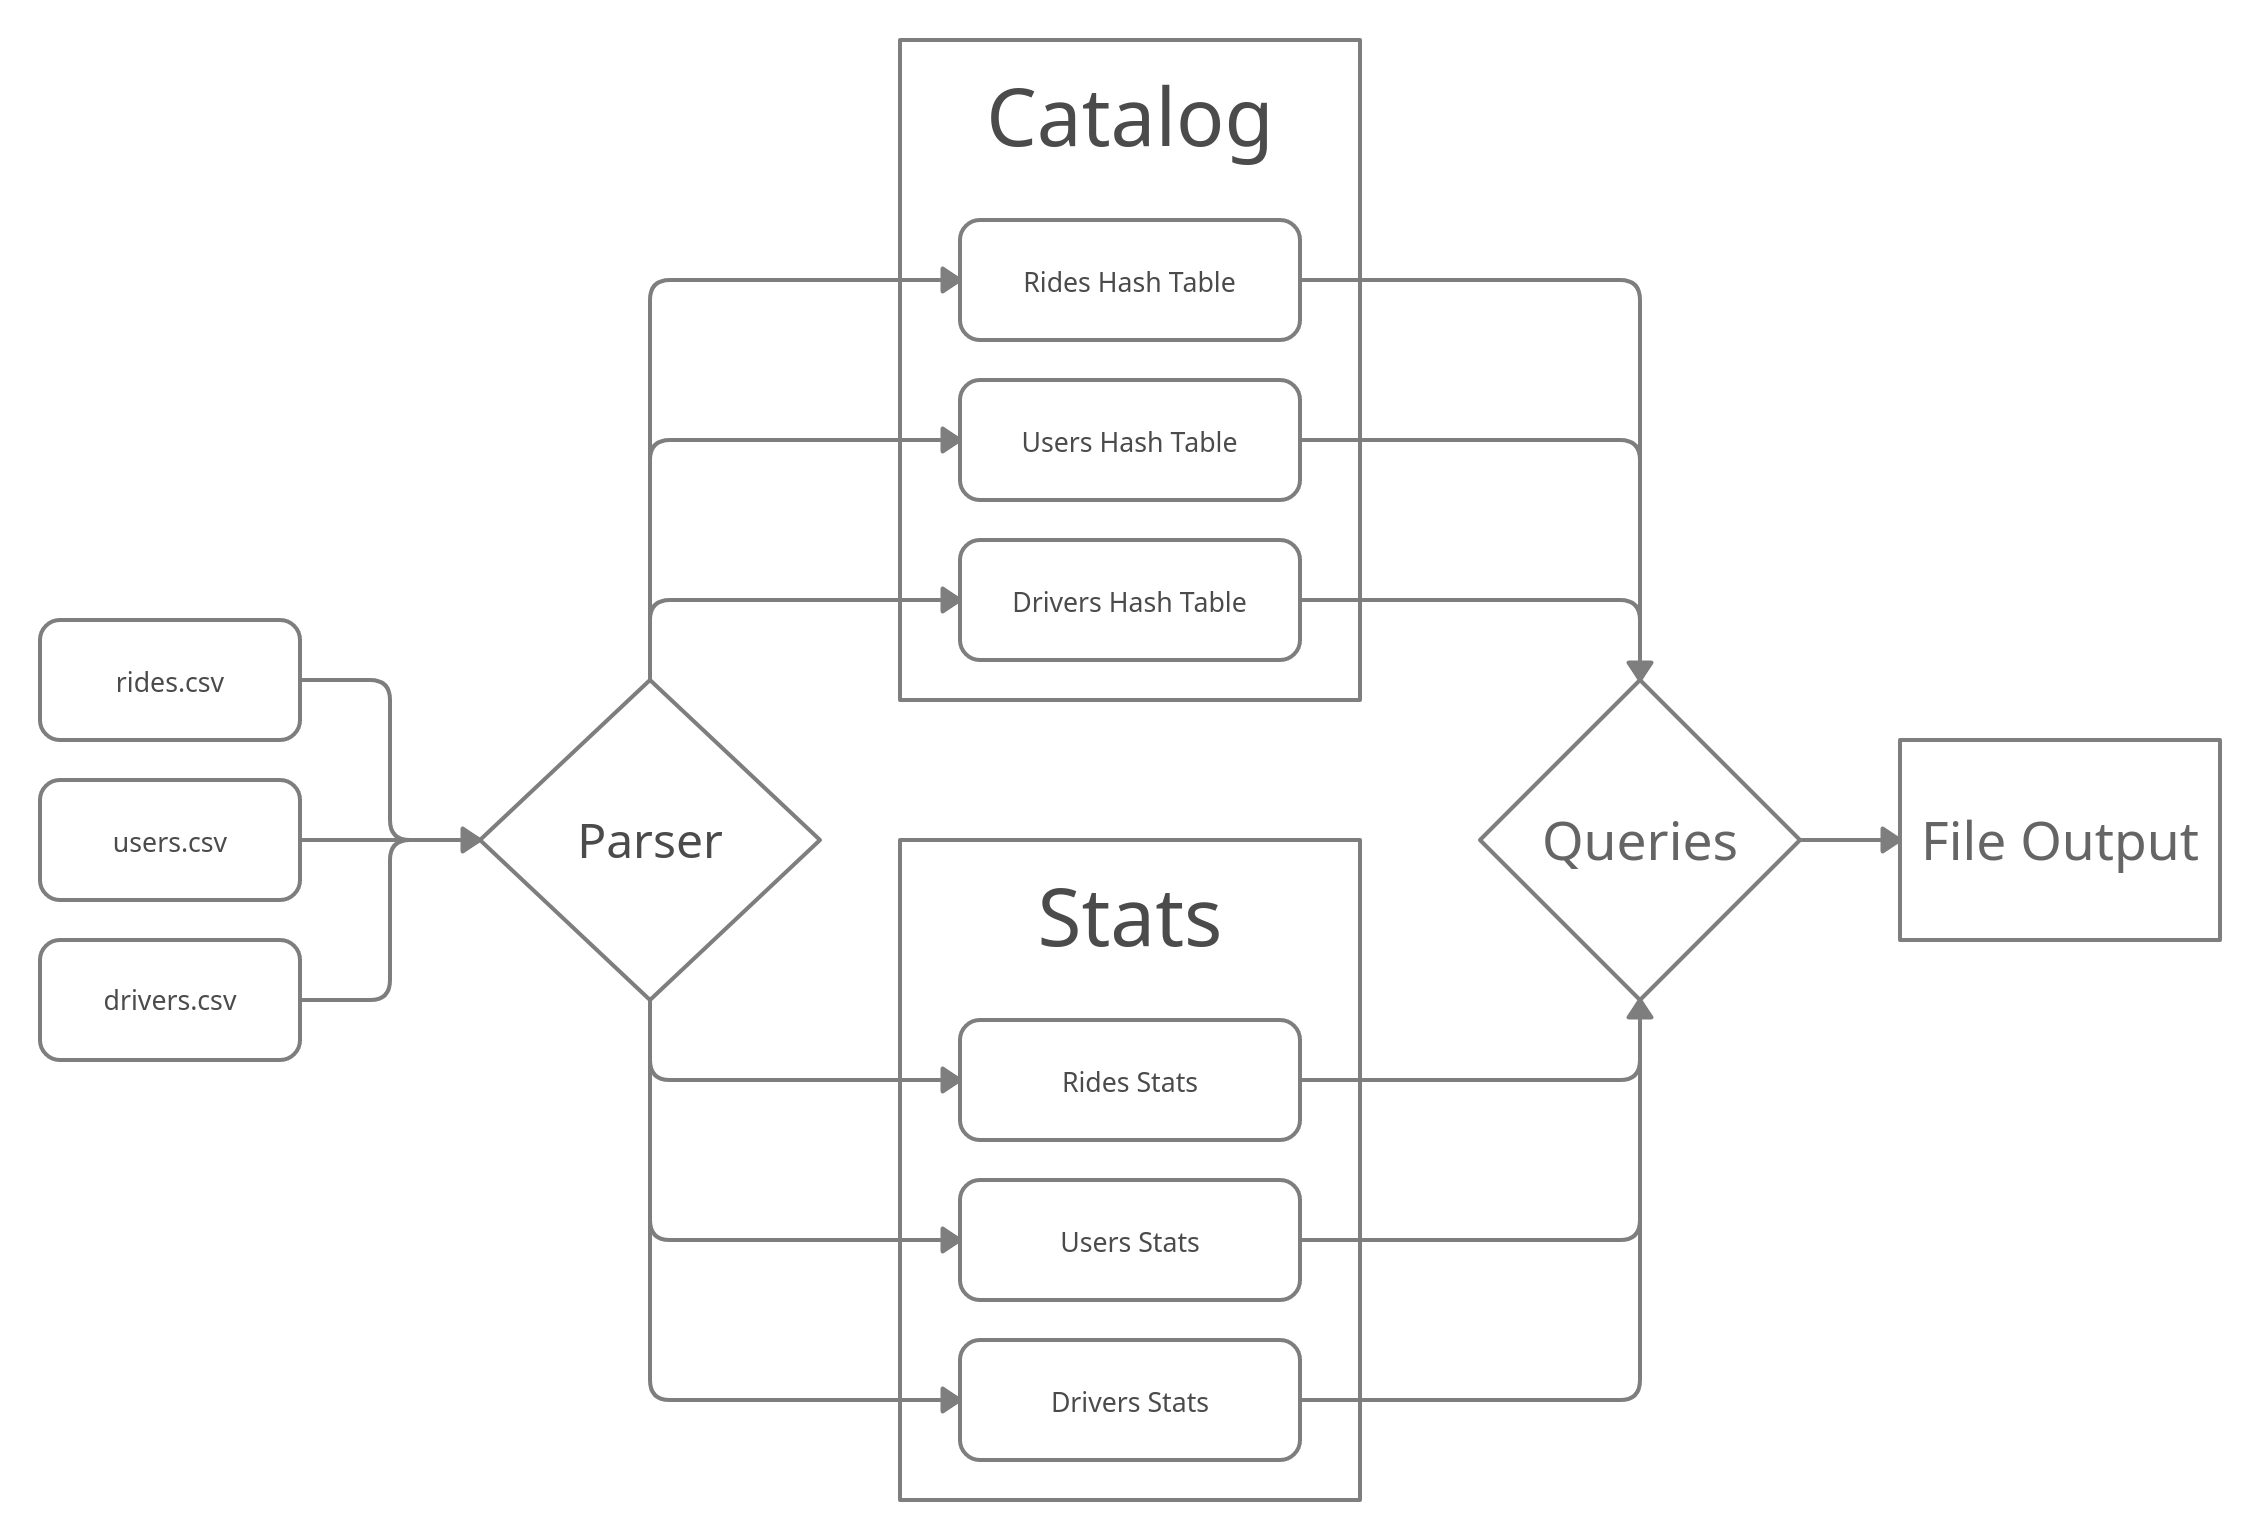
\includegraphics[scale = 0.14]{diagram1.png}
    \centering
    \caption{Diagrama da estrutura utilizada para o projeto}
    \end{figure} \\
    Depois disto chegou a hora, então, de partir para a ação. O desafio inicial foi perceber quais as estruturas ideais para armazenar todos os dados. Concluímos que \textit{hash tables} eram o ideal para as estruturas principais, uma vez que apresentam tempo de acesso (\textit{lookup}) constante. Criamos, portanto, três \textit{hash tables} - uma para os \textit{users}, uma para os \textit{drivers} e outra para as \textit{rides}. De modo a assemelharem-se ao máximo a uma base de dados, decidimos (seguindo a arquitetura descrita em cima) agrupá-las todas numa estrutura \textit{mãe} apelidada de catálogo, onde cada uma das \textit{hash tables} seria uma tabela da base de dados. Após isto foi necessário pensar no \textit{parsing} dos dados. Desenvolvemos uma solução bastante simples, pois como o input se trata de um ficheiro CSV unicamente separado por pontos e vírgulas, criamos um parser geral que poderia ser chamado por outras funções noutro ficheiro que sabem assim utilizar o output do parser, contribuindo assim para a modularização do código. Definimos assim o módulo \textit{parser} de forma ao mesmo não ter noção dos dados que está a receber - isto foi alcançado com recurso a \textit{function pointers}, um recurso muito interessante e útil de C. \\
    \begin{figure}[h]
    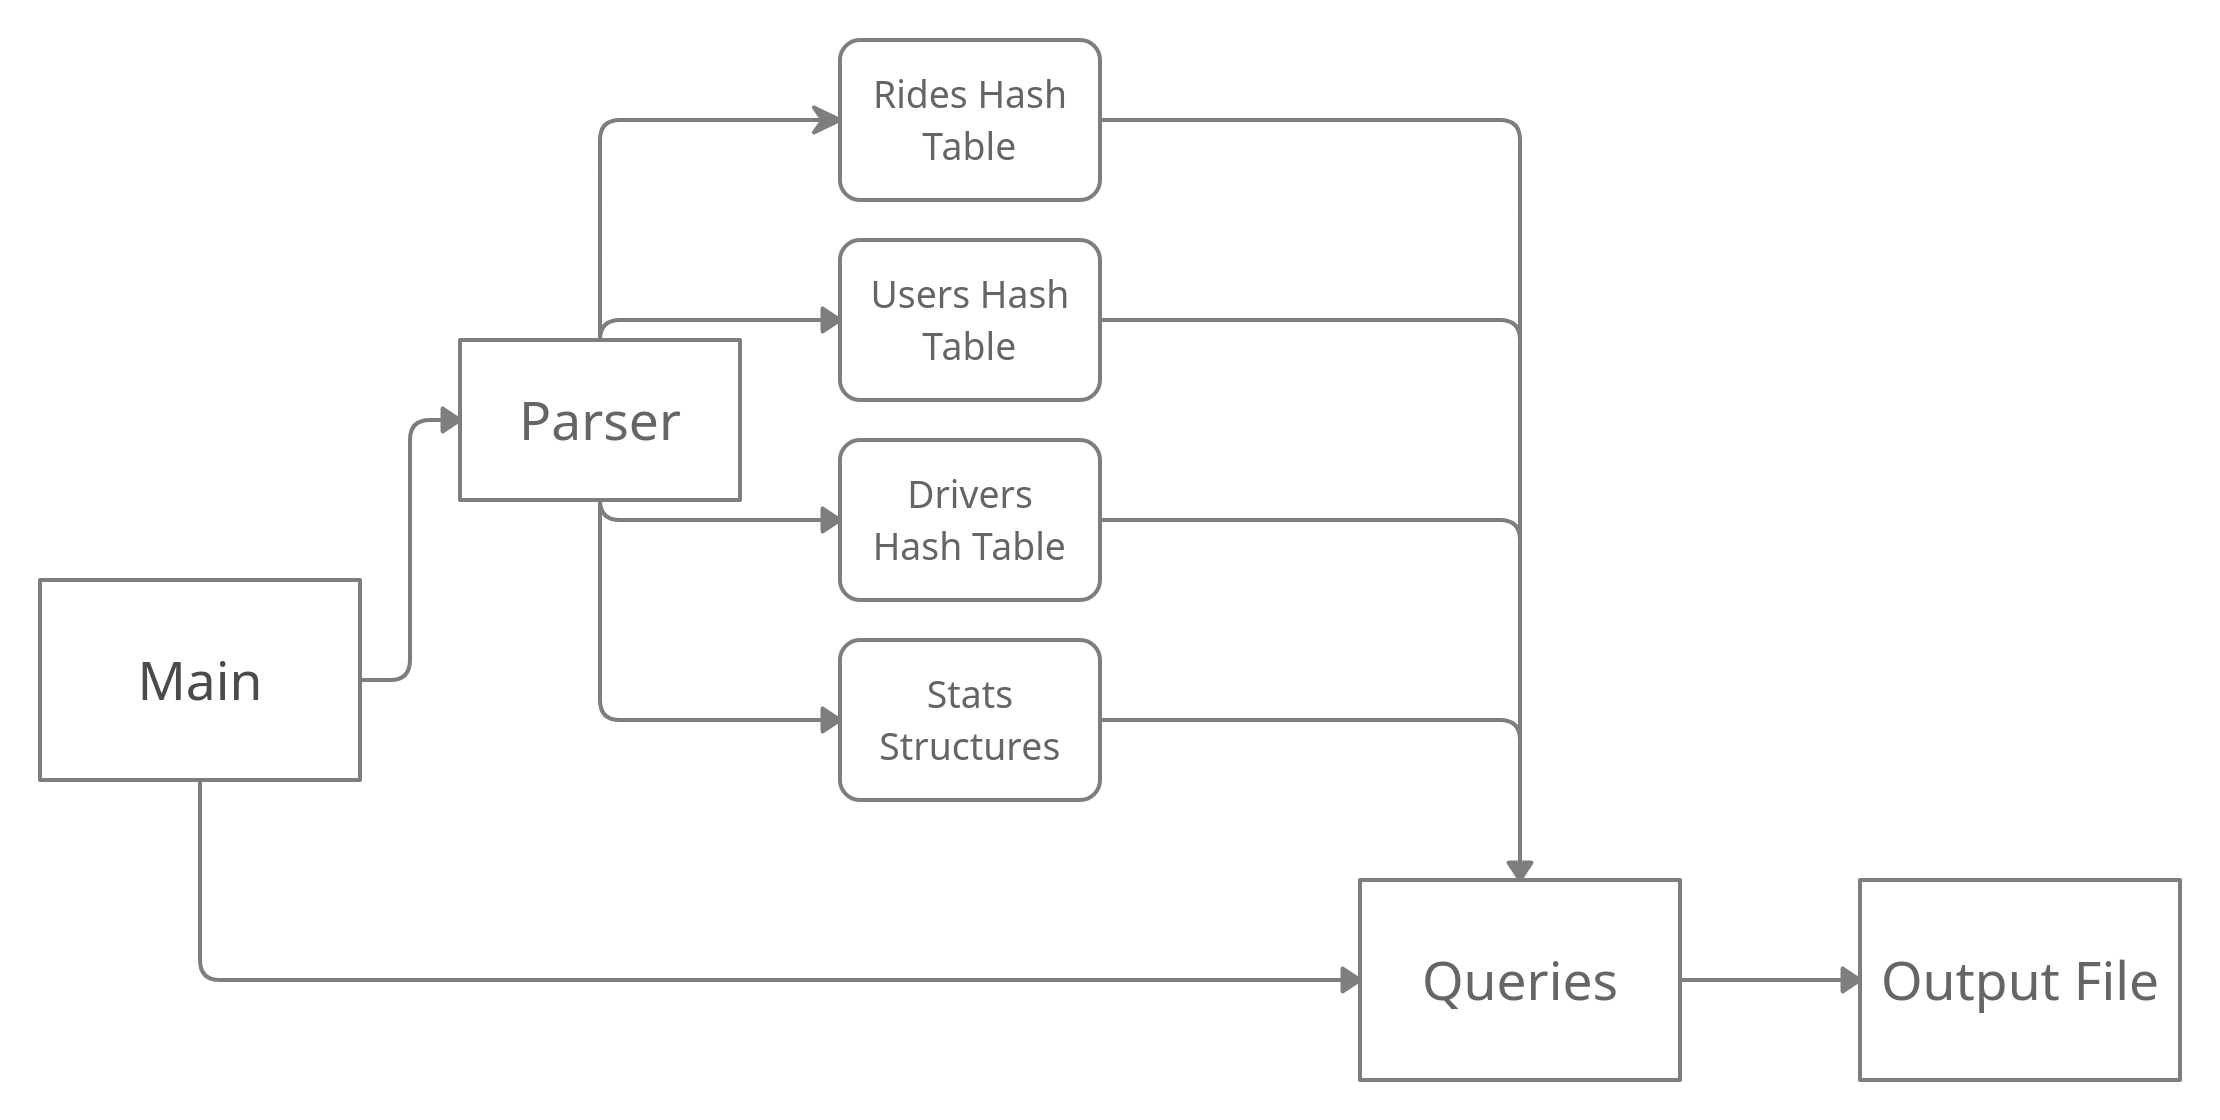
\includegraphics[scale = 0.15]{diagram2.png}
    \centering
    \caption{Diagrama do funcionamento do programa}
    \end{figure} \\
    Finalmente, de forma a finalizar o solicitado nesta primeira fase, optamos por escolher responder às três primeiras queries. Isto pois, no nosso ponto de vista, eram aquelas cuja implementação era mais simples. \\
    Assim, passaremos a explicar a forma como implementamos cada uma das três: \\
    \textbf{Query 1}: Esta primeira query consiste em \textit{"listar o resumo de um perfil registado no serviço através do seu identificador"} - onde os identificadores são o \textit{username} para os \textit{users} e o \textit{id} para os \textit{drivers}. Tomemos como exemplo as seguintes linhas: \\
    1. \textit{1 MiRibeiro33} (query destinada a um \textit{user}) \\
    2. \textit{1 000000000024} (query destinada a um \textit{driver}) \\ 
    Assim sendo, o que fez mais sentido foi colocar estes identificadores como chave de cada uma das \textit{hash tables} das entidades referidas, aproveitando assim o tal \textit{lookup} constante. A partir daí, foi só construir o perfil da entidade solicitada. A maioria da informação que é impressa está diretamente armazenada nas \textit{hash tables} dos utilizadores/drivers, mas o total gasto/auferido e o número de viagens realizadas têm de ser calculadas com base nos dados das \textit{rides}. É aqui que as estruturas do módulo \textit{stats} nos ajudam. Uma vez que guardamos todos estes valores numa estrutura auxiliar durante o \textit{parsing} do ficheiro, precisamos apenas de acessá-los diretamente, trocando algum tempo de \textit{startup} por muita poupança. Um \textit{tradeoff} que é realizado em várias implementações do nosso projeto.
    \\
    \textbf{Query 2}: A segunda query consiste em \textit{"listar os n condutores com maior avaliação média"}, contando com vários critérios de desempate - em caso de empate em relação à avaliação média deverá aparecer o condutor com a viagem mais recente primeiro e, em caso de novo empate, deverá ser usado o \textit{id} do condutor por ordem crescente. Decidimos implementar uma \textit{linked list} que guarda as estatísticas de um condutor e que é atualizada durante a inserção das \textit{rides}.
    Esta opção foi tomada porque a inserção e a ordenação (o algoritmo utilizado foi o \texttt{quick sort}) são mais rápidas numa \textit{linked list}. Ainda assim, a mesma apresenta dois problemas: ocupa mais memória e apresenta baixa localidade espacial. Portanto, no futuro, iremos repensar a nossa escolha e, provavelmente, implementar um \textit{array}.
    \\
    \textbf{Query 3}: A terceira query consiste em \textit{"listar os n utilizadores com maior distância viajada"}, contando novamente com vários critérios de desempate - em caso de empate em relação à distância viajada, deverá aparecer o utilizador com a viagem mais recente primeiro e em caso de novo empate, deverá ser usado o \textit{username} do utilizador por ordem crescente. É de notar que esta query é bastante parecida à segunda e, portanto, após implementarmos a segunda, a implementação desta foi trivial. É de esperar também que a estrutura usada nesta se assemelhe à usada na segunda. Assim sendo, novamente, tomamos a opção de implementar uma \textit{linked list}.

\newpage

    \chapter{Dificuldades sentidas}
    Como já referido este trabalho não é fácil, o que implica que existiram e existirão muitas adversidades associadas. A maior dificuldade foi, sem dúvida alguma, a implementação cuidadosa do encapsulamento e da modularidade. Reconhecemos que estes pilares são fundamentais para um programa de qualidade, mas achamos que C não é a linguagem ideal para tal. Uma linguagem como Java, onde o paradigma é orientado a objetos, seria muito superior neste quesito. A facilidade de poder definir \textit{atributos e métodos} públicos ou privados é um \textit{must}. De qualquer das formas, acabamos por conseguir implementar os mesmos em grande parte do projeto. Ainda assim, consideramos que, por exemplo, a forma como atualizamos os dados dos \textit{users} e dos \textit{drivers} (ao mesmo tempo que lemos os dados das \textit{rides}) pode, eventualmente, quebrar o encapsulamento. A realidade é que o tópico do encapsulamento é bastante extenso e complexo e, uma vez que é a primeira vez que o estamos a abordar, existirão, naturalmente, falhas. Fica aqui o dever de melhorar este aspeto na segunda fase. \\
    Outra das dificuldades sentidas foi o facto de realizarmos mudanças atómicas no código sem perceber se estávamos a \textit{partir} algo noutra parte do código. É de notar que um dos pontos levantados pelo encapsulamento e modularidade é a \textit{garantia} de realizar estas mudanças sem grandes problemas associados - o que prova que, provavelmente, não implementamos os mesmos da forma mais eficaz. De qualquer das formas, uma maneira de contornar este problema foi criar testes unitários de apoio às \texit{funções} criadas (testes estes executáveis a partir do comando \texttt{make test}). Apesar disto não ter peso aparente na nota do projeto pretendemos continuar a aplicá-los - já que demonstraram grande sucesso até agora.
    
\newpage

    \chapter{Aspetos de desempenho}
    Neste capítulo iremos abordar alguns aspetos de desempenho relacionados a estas três primeiras queries que foram implementadas. Achamos que um dos aspetos mais importantes nos programas de hoje em dia é o tempo de execução de um programa. Tomemos como exemplo a seguinte lista de queries. 
    \begin{verbatim}
        1 PetrPacheco
        1 VaCosta
        1 LeTavares103
        1 000000002639
        1 000000008561
        1 000000004987
        2 50
        3 50
    \end{verbatim} 
    Portanto, seis queries do \textit{tipo} 1 (três delas destinadas a \textit{users} e três delas destinadas a \textit{drivers}), uma query do \textit{tipo} 2 e uma do \textit{tipo} 3. \\
    Em baixo, apresentamos os resultados do tempo de execução, sobre a lista dada, em três diferentes máquinas. \\
    \begin{tabular}{|c||p{4cm}|p{4cm}|p{4cm}|}
    \hline
    & Máquina 1 & Máquina 2 & Máquina 3 \\
    \hline
    CPU & Intel Core i5-8300H & Apple M1 & Ryzen 7 5800U \\
    \hline
    Cores/Threads & 4/8 & 8/8 & 8/16 \\
    \hline
    RAM & 16GB DDR4 2666 & 16GB DDR4 2666 & 16GB LPDDR4 4200 \\
    \hline
    Disco & 512GB SSD M.2 & 512 GB SSD M.2 & 512GB SSD M.2 \\
    \hline
    OS & Arch Linux & macOS Monterrey & Arch Linux \\
    \hline
    Tempo & 1,635s & 1,135s & 1,580s \\
    \hline
    \end{tabular}
    \caption{ \label{demo-table} \begin{center}\footnotesize Nota: O tempo foi obtido realizando os testes 10 vezes, removendo o pior e o melhor resultado, e calculando a média dos 8 restantes. \end{center}} 
    \noindent Os tempos obtidos da máquina 1 e da 3 foram bastante semelhantes, devido a ambas usarem a mesma arquitetura base (x86) com frequência semelhante, tendo a máquina 3 uma pequena vantagem entre os dois, apesar do menor consumo de energia devido a ser um processador mais recente com um processo de fabricação menor, e, deste modo, mais eficiente (14 vs 7nm). \\
    No entanto, nenhum dos dois se equipara à performance do MacBook com o processador M1 projetado na arquitetura ARM, cujo tempo de execução é aproximadamente 30\% menor que ambos os computadores x86. Esta diferença deve-se à performance \textit{single-core} ser muito superior neste processador e ao facto de ainda não termos suporte a \textit{multi-threading} no programa, cuja implementação iria diminuir a disparidade, devido tanto às limitações energéticas e térmicas do MacBook, como à existência de muitas mais threads na máquina \textit{Ryzen}. Deste modo, implementar \textit{multi-threading} é algo que pretendemos no futuro. \\
    Em termos de memória, foi atingido um pico de 370 \textit{megabytes}, algo pouco significante tendo em conta o tamanho dos dados inseridos e bem abaixo do limite de 2GB pedido pelos docentes, mas é algo que trabalharemos para reduzir caso seja um problema com os ficheiros de maior dimensão da 2ª fase.
\newpage

    \chapter{Conclusão}
        Em suma, apesar das várias dificuldades e novos desafios colocados por este projeto, pensamos estar à altura deste problema, e que no planeamento fizemos as decisões certas e por isso conseguimos construir uma boa base a partir da qual conseguimos expandir e alterar para as \textit{queries} mais complexas da 2ª fase. Sendo assim, sentimo-nos preparados para concluir o projeto e melhorar ainda mais o que já fizemos até agora, sendo que o que já completamos ensinou-nos muito sobre alguns aspetos da programação que tínhamos abordado menos, como a modularização e encapsulamento, sendo estes princípios fundamentais para criar código sustentável e seguro, sendo assim essencial fomentar estes conhecimentos nos alunos.
\end{document}